\chapter{设备描述与性能}
\section{背景}
用于获取本篇报告中的数据的所使用设备耗时两年多的时间研发出来。

1967年间,为了定位、评估高放射性本底区域的放射性材料的数量,Blumberg、\newline Mauney和Scott \footnote{R.\ Blumberg,T. H. Mauney, and D. Scott, MSR Program Semiannu. Progr. Rep. Aug. 31, 1967, ORNL-4191, pp.40-44.} 开始研究这样的设备。1967年MSRE停堆期间,他们使用一个悬挂在可移动的维护屏(PMS)中的准直器的$\gamma$ 射线计量仪,描绘出来自热交换器的发射性强度。以此同时,使用NaI晶体闪烁探测器获得了一些能谱数据。在1968年三月,他们制造出更好的$\gamma$能谱探测器,此探测器包括:一组不同准直屏蔽组件,一个Ge(Li)半导体和400道多道分析仪\footnote{R.\ Blumberg,F. F. Dyer, and T. H. Mauney, MSR Program Semiannu. Progr. Rep. Aug. 31, 1968, ORNL-4344, pp.36-40, 196.}。本文的结论是通过带有准直束的$\gamma$ 能谱仪远程测量裂变产物沉积物是可行的。不过,也有以下几个方面需要改进\footnote{R.\ Blumberg,F. F. Dyer, and A. Houtzeel, MSR Program Semiannu. Progr. Rep. Aug. 31, 1969, ORNL-4449, pp.31.}:
\begin{enumerate}
\item 提高设备对选定区域的定位、准直精确能力。
\item 从多种核素中辨别出各个核素,探测器要有好的分辨率。
\item 简化对数据的处理、分析。
\item 测量大范围放射源强度时,准直器可调。
\item 支持在堆运行期或停堆时对堆选定点的能谱测量。
\item 更好的刻度方法。
\end{enumerate}
\noindent 到1969年六月,上述的目标已经基本实现。

\section{概括性描述}
如图\ref{Fig_1_3}所示,燃料循环系统和排泄槽位于地下单元,堆运行期间,这个单元将被一个不锈钢薄片包着的水泥墙覆盖住。当堆满功率运行时,堆单元的$\gamma$放射性水平在40000-70000\ R/hr(琴伦每小时,表征射线的照射率)之间;当停堆排出熔盐时,降到3000-5000\ R/hr,然后缓慢地下降\footnote{A.\ Houtzeel, MSR Program Semiannu. Progr. Rep. Aug. 31, 1968, ORNL-4344, pp.22-23.}。在熔盐排入排泄罐后,这里的$\gamma$放射性立即达到25000\ R/hr。因此,任何的$\gamma$能谱测量都是通过屏蔽体的狭缝进行的,距离在10-20\ ft(ft为英尺1\ ft=304.8\ mm)左右。

即使在屏蔽体顶部,通过孔隙的$\gamma$射线强度也是十分高的。例如,在停堆、排料的一至两天后,可移动的维护屏蔽体中超过5英寸的直径的小孔和离热交换器14英尺地方测到的强度在500\ R/hr水平。因此,到探测器的放射性活度不得不用准直器削弱,或有时也屏蔽体。当然,射束准直器必须限制定位在要分析的$\gamma$\ 射线源方向上。

\begin{figure}
%\graphicspath{{Figure/}}
\centering
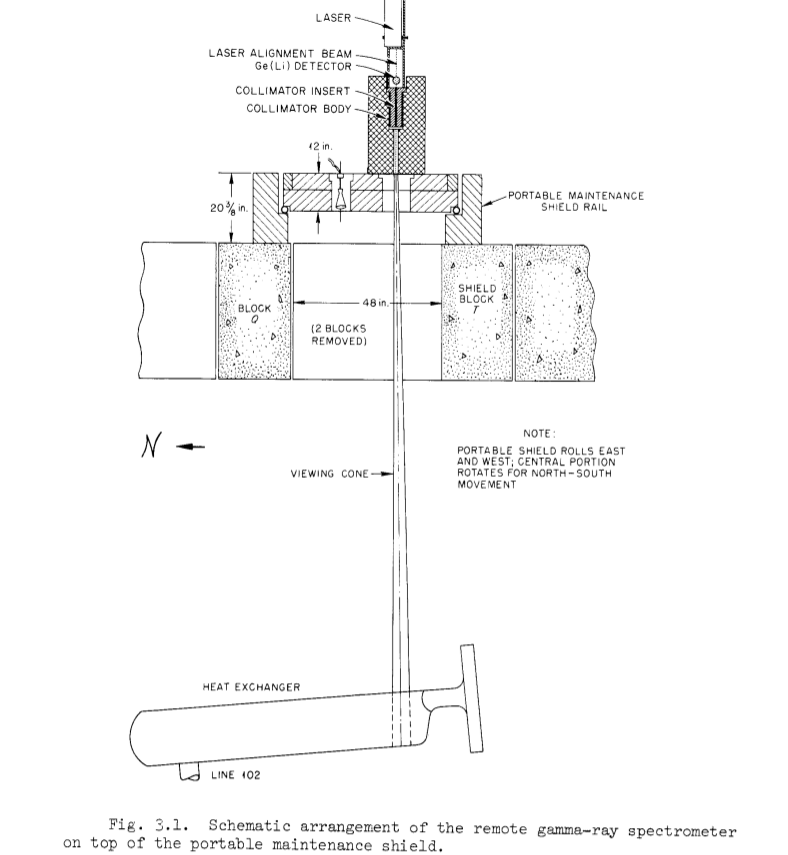
\includegraphics[width=0.8\textwidth]{Fig_3_1}
\caption{Schematic arrangement of the remote gamma-ray spectrometer on top of the portable maintenance shield.}
\label{Fig_3_1}
\end{figure}
图\ref{Fig_3_1}是这套设备的正面示意图,包括一个准直器、一个探测器和一个激光准直设备。图\ref{Fig_3_2}是设备的正视图实物图。在此图解中,这套设备被安置在可移动维护屏之上,但它也可以安置在钻有小洞的混泥土屏蔽罩上面。探测器是Ge(Li)晶体,连接适当的放大器到一个4096道的多道分析器。这样组合提供了高分辨率的能力。依赖$\gamma$射线强度,可以选择不同的嵌入式准直器。在可移动维护屏上使用这套设备时,通过激光准确定位测量的区域,透过可移动维护屏上的铅玻璃窗观察堆中的定位部位。这样可以通过移动可移动维护屏,达到精确定位。

\begin{figure}
%\graphicspath{{Figure/}}
\centering
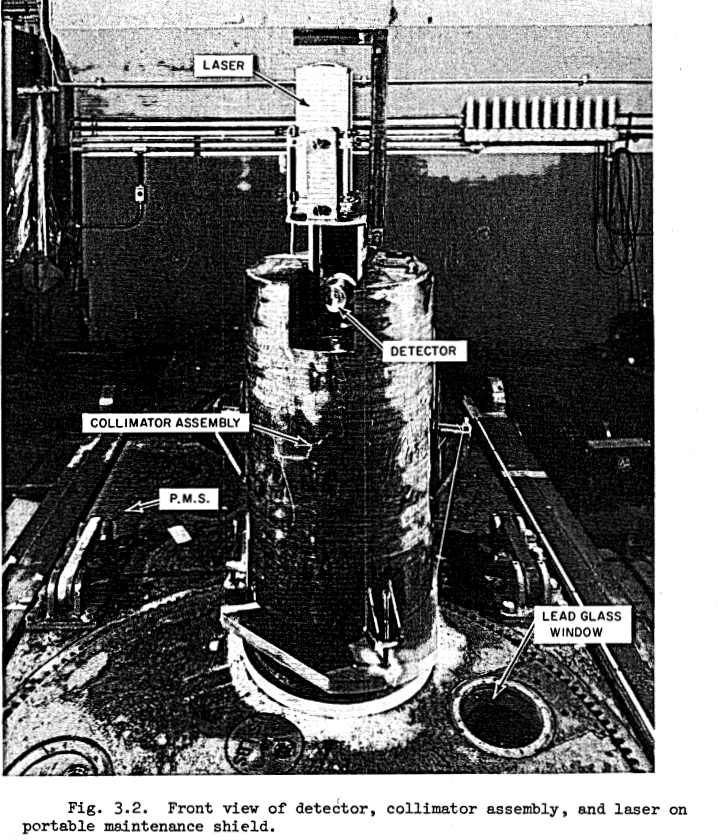
\includegraphics[width=0.8\textwidth]{Fig_3_2}
\caption{Front view of detector,collimator assembly, and laser on portable maintenance shield.}
\label{Fig_3_2}
\end{figure}

\section{探测器与前置放大器}
探测器是一个ORTEC公司制造的同轴锂漂移锗探测器,1333\ keV峰位的分辨率为1.78\ keV,直径36.65\ mm,长28.5\ mm,有效灵敏体积26.25\ $cm^3$,峰康比27/1。相对效率为4.3\%。配套ORTEC-440A或ORTEC-450放大器。

虽然到达探测器的准直射线强度挺强的,但是实际上和锗晶体发生作用的还是很少的。虽然设备并非在理想状态下用六个月的时间获得1400个能谱,但是整个系统的分辨率却没有变差。

\section{多道分析器}

使用Nuclear Data 2200系列4096道的多道分析器,所有谱保存到磁带。起先在操作分析器和磁盘时都会遇到一些问题,这些都是由于系统漏洞导致的。把多道分析器放置在一个高温且潮湿的环境中都会出现问题,使得系统在实验期间经常当机。

一旦把分析器和放大器放到控温、控湿的房间时,大部分问题都得到解决。用一条200ft的电缆连接前置放大器和主放大器,这么长的电缆对系统的系能影响可以忽略。由于当地供电系统不稳定(电压、频率不稳定),系统增益有时会有几道的漂移。高分辨率的探测器和4096道分析器满足当下的实验要求。反应堆运行时,一些堆组件(如热交换器、排气系统)中短寿命的裂变产物放射出的$\gamma$\ 射线杂音太多,导致能谱出现严重的重峰问题。这种情况下,在探测器和被测量区域之间加入适当的屏蔽来降低放射性强度,或者这样的谱不做处理。

\section{准直组件}

图\ref{Fig_3_3}展示了准直组件,其包括准直体、准直内插件,材质均为铅。准直体高32.5\ in,直径19\ in,中间有个圆孔用于嵌入准直内插件,准直内插件有三种不同孔径规格,分别位1/16、1/8、3/16\ in。

探测器和杜瓦瓶固定在准直体上的一个平台上,并可做微调处理。顶部的激光发出的光束通过准直内插件的准直孔,达到精确定位,在激光定位时,探测器和杜瓦瓶需要从准直组件上移出,也可以在不移动探测器和杜瓦瓶的情况下,通过一套复杂的光学系统达到精确定位。

\begin{figure}
%\graphicspath{{Figure/}}
\centering
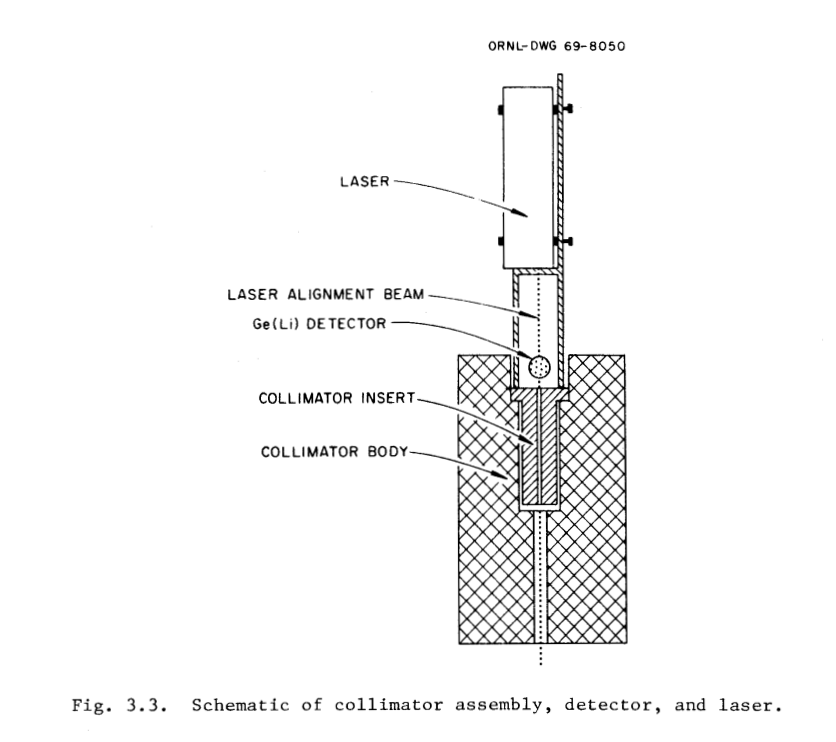
\includegraphics[width=0.8\textwidth]{Fig_3_3}
\caption{Schematic of collimator assembly, detector, and laser.}
\label{Fig_3_3}
\end{figure}

\section{实验设备安装}

停堆之后,需要花费几天的时间移出上层的屏蔽块和阻隔板,然后安装PMS和探测器装置。这种方式太长时间,所有决定在堆排气系统、主热交换器和排泄罐这三个需要观察的区域的屏蔽层打孔,这样就不用移动屏蔽层。在1969年停堆期间,打好这些孔。孔的校准通过人力移动上下屏蔽层,使其排成一条直线。把探测器和准直组件安置在屏蔽层上面,当停堆时,设备可立即工作,至少在这三个区域,就有机会研究较短寿命的核素。

使用PMS沿着热交换器轴线、燃料管路和排气管路观察裂变产物的放射性活度\footnote{R.\ Blumberg and E. C. Hise, MSRE Design and Operations Report.Part X. Maintenance Equipment and Procedure, ORNL-TM-910.}。图\ref{Fig_3_4}展示整个设备全貌。探测器和准直器安装在一个大的转盘上,因此能在PMS上自由转动。

\begin{figure}
%\graphicspath{{Figure/}}
\centering
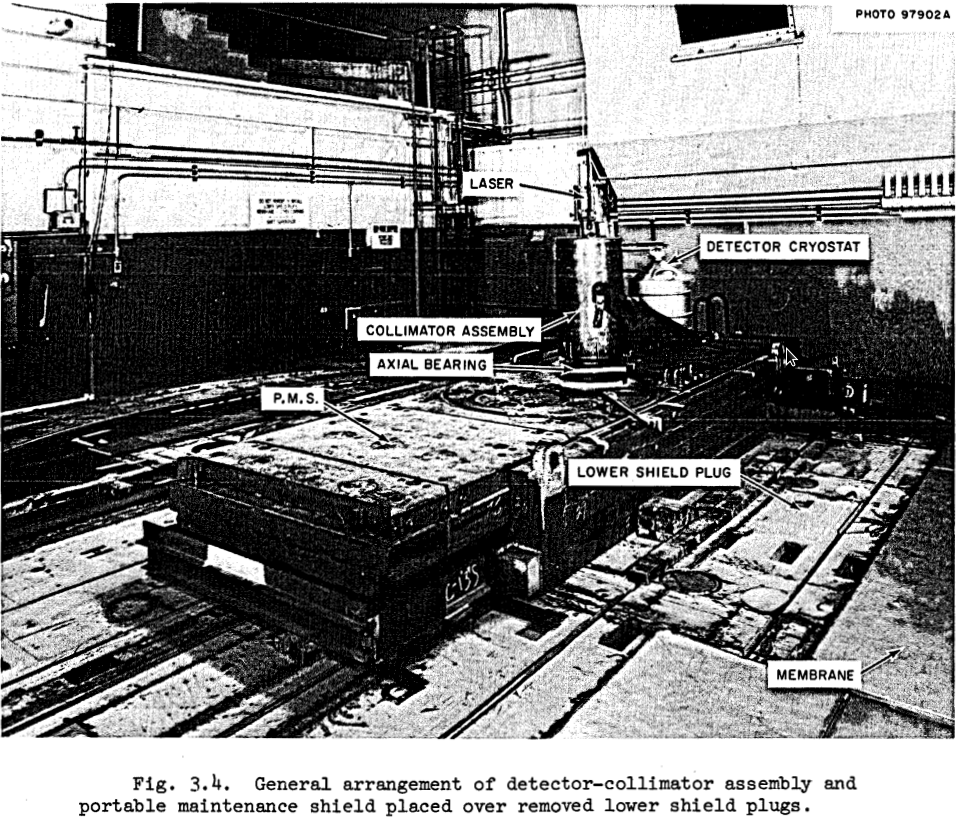
\includegraphics[width=0.8\textwidth]{Fig_3_4}
\caption{General arrangement of detector-collimator assembly and portable maintenance shield placed over removed lower shield plugs.}
\label{Fig_3_4}
\end{figure}

\section{定位设备}

精确定位获取$\gamma$\ 谱的组件位置是很重要的,本实验用一个低能激光和两个测量员的搬动实现这个目的。激光器固定在可调动的准直内插件上,激光束通过准直器中心孔洞,照射在将要测量$\gamma$能谱的位置上,出现一个红色斑点,这可以通过PMS上面的铅玻璃窗观看到。事先通过铅垂直线和水平仪调整,保证准直体水平,且激光束垂直。再配合测量员移动活动区,这样使定位系统精度达到1英寸以内。

\section{屏蔽}

如上面提到的各个堆组件,都有很强的放射性。当堆在运行期间,从覆盖在堆排气系统和热交换器之上的水泥屏蔽层的小孔测得的强度高于1000 R/hr。还有由快热中子引发的照射剂量。(除非采谱时,孔被堵塞,并用铅砖盖住。)

当堆满功率运行时,已经被证实不可能从热交换器上获得有用的$\gamma$谱图。熔盐回路中的很多裂变核素的光电峰叠加在一起,且偶然符合效应也产生很多无用的大叠加峰。计算程序就无法从这样的能谱分析出有用的信息。排气系统里所包含的核素种类比熔盐燃料少得多,但即使这样,反应堆满功率运行时在排气系统上测得的谱也是几乎没什么价值。为了得到排气系统上有用的谱图,需要使用一些屏蔽材料,如2英寸厚的浸有锂的煤油和1英寸厚的铜。(煤油中的锂用于吸收中子而不会发射出$\gamma$射线。)

当反应堆低功率运行或停堆时,就可以从热交换器和排气系统采谱分析。但仍然需要适当的屏蔽来保证探测器的输入计数率在合理的范围内,如3000-10000\ counts/sec。

现在面临的问题是需要许多好的屏蔽材料,如铅能大大降低低能$\gamma$\ 射线(能量低于几百keV)的强度,足够的铅屏蔽对更高能量的光子的强度也会有适当的减弱。因此,在这样的情况下,低能峰完全可以被屏蔽掉。由于低原子序数材料对低能$\gamma$射线没有好的屏蔽效果,铝或铜制的屏蔽可以克服这个缺点。从而,计数率可保持在一个理想的水平,同时允许较低能的$\gamma$射线测量。关于设备的刻度在第五章会有比较详细的描述。

通常,我们使用最少的屏蔽擦料和1/16\ in.规格的准直内插件,控制探测系统的死时间在低于25\%的水平下工作。

\section{刻度设置}

\begin{figure}
%\graphicspath{{Figure/}}
\centering
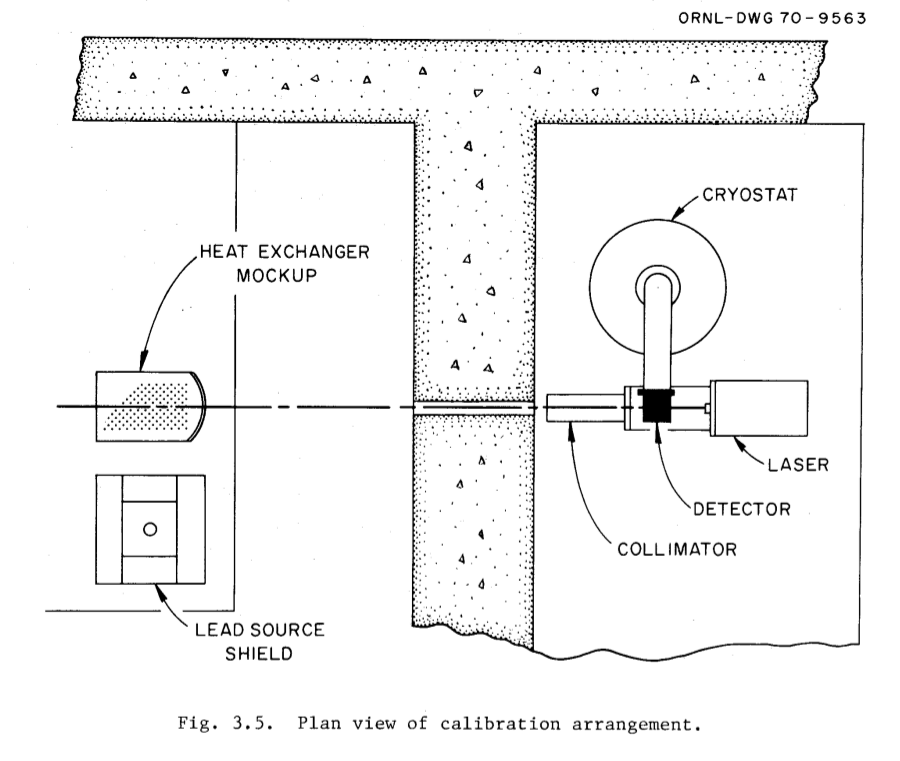
\includegraphics[width=0.8\textwidth]{Fig_3_5}
\caption{Plan view of calibration arrangement.}
\label{Fig_3_5}
\end{figure}

探测系统的效率是通过经验方式确定的,特别是热交换器的几何结构过于复杂,而无法通过理论计算来确保足够的精确。第五章将会给出复杂的刻度过程。附录D用简单的计算模型做了验证。

图3.5展示刻度实验的物理装置。探测器和一个准直器被安装在堆high-bay area中的一个地下单元(净化单元)。一个携带着放射管源的完整的主热交换器模型位于相邻的远程维护实践单元。固定在热交换器里面的放射源放出的射线穿过墙上的小孔和准直器,并和探测器相互作用。这堵墙足够厚,射线只能从准直器的小孔到达探测器。除了与模型直接接触的空间外,远程维护实践单元用普通的顶盖封闭;在此也用到PMS。通过PMS上的小孔,我们就可以借用简单的工具操作模型中的放射源和模拟热交换器的管子。

刻度实验中使用了活度24\ Ci(居里)$^{110m}$Ag 放射源。此放射源长6.3 in,直径0.5 in(真实的热交换器管道也是同样的直径),由橡树岭研究堆辐照活化得来。

使用设计的探测器测量此放射源放在热交换器模型的各个位置的放射性强度,这样就能得到热交换器各个点对探测器的响应情况。热交换器模型与探测器之间的距离与真实的热交换器和安装在PMS上的探测器的距离相当。

由于反应堆中的主排气线是一个直径1英寸的波纹管,对它刻度相对比较简单。通过对比放射源的管子,就可估计出它的刻度。

热交换器上的陶瓷部件以及为了如实观察热交换器和排气线而用到的屏蔽块也用相同的源做了刻度,估计其屏蔽能力,并与文献提供的数据计算做比较。为了达到目的,陶瓷发热器紧挨着放有管状放射源的热交换器的未屏蔽中心位置上。屏蔽块也是和远程维护实践间正面有孔的墙紧紧贴着。不同的屏蔽块的屏蔽能力和文献提供的计算结果符合。
